\begin{frame}{What is a Microcontroller?}
    \par Microcontroller is a computer system in a single chip.
    \par Just like a \acs{pc}, it consists of:
    \begin{itemize}
        \item \acs{cpu} --- less powerful than a full blown desktop processor
        \item Persistent and non-persistent memory (\acs{hdd}, \acs{ram}) --- typically a few \SI{100}{\kibi\byte} of \acs{ram} instead of > \SI{1}{\gibi\byte} like a typical computer
        \item System clock --- not as fast as desktop processors, but many \acsp{uc} can also be clocked externally
        \item Peripherals --- provide interfaces found in the field of embedded systems (\acs{gpio}, \acs{i2c}, \acs{spi}, \acs{uart}, \acs{can}, \ldots) rather than interfaces found in desktop computers (\acs{pci}, \acs{pcie}, Thunderbolt \texttrademark, \acs{sata}, \ldots)
    \end{itemize}
\end{frame}

\begin{frame}{What is a Microcontroller?}
    \begin{figure}
        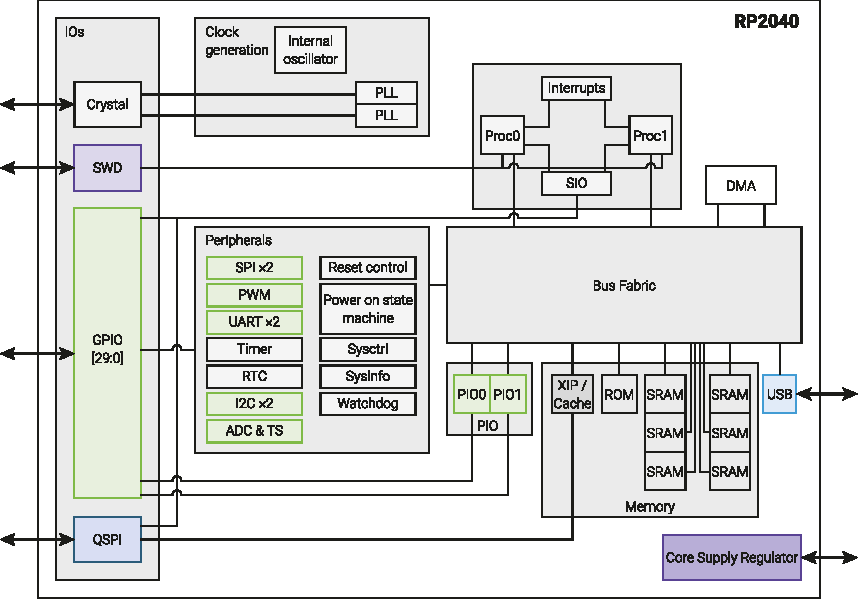
\includegraphics[width=0.9\textwidth]{microcontroller/arduino/rp2040/block-diagram.pdf}
        \caption{System overview of the RP2040 Chip}
    \end{figure}
\end{frame}

\begin{frame}{What is a Microcontroller?}
    \begin{figure}
        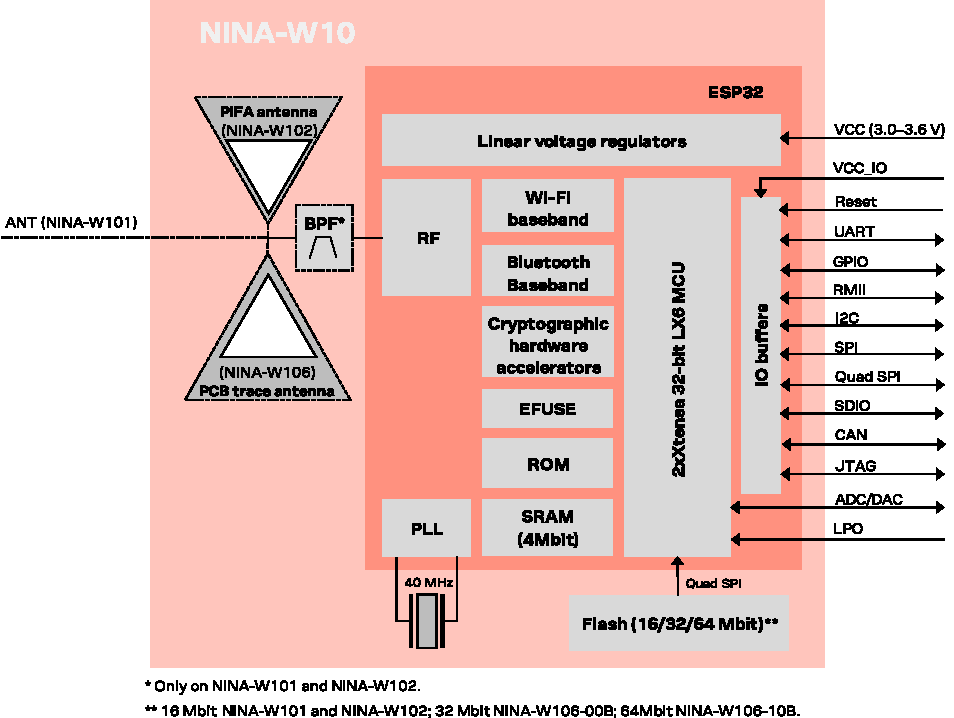
\includegraphics[width=0.9\textwidth]{microcontroller/nina-w10-block-diagram.pdf}
        \caption{Nina W10 Block Diagram}
    \end{figure}
\end{frame}

\begin{frame}{What is a Microcontroller?}
    \begin{figure}
        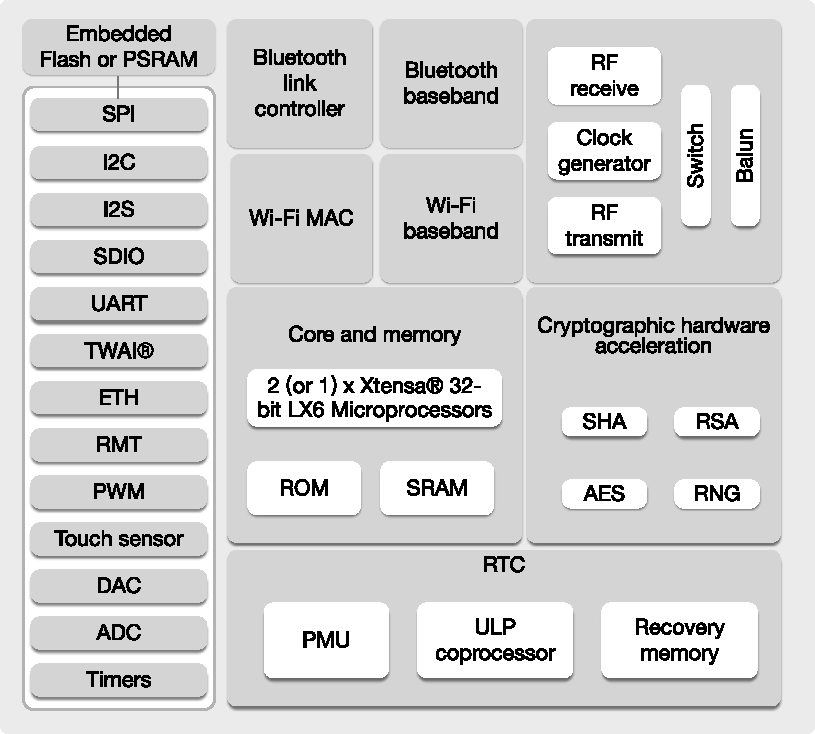
\includegraphics[width=0.7\textwidth]{microcontroller/esp32-functional-block-diagram.pdf}
        \caption{ESP32 Functional Block Diagram}
    \end{figure}
\end{frame}